\section{The argument against neutrality}
\label{sec:arg}

\begin{Theorem}{The argument against neutrality}{}
The intuition of neutrality (Def.~\ref{def:ion}) is incorrect.
\end{Theorem}

The \emph{argument against neutrality} (described in \citeNP[p.~176f]{broome_2012}) concludes that the intuition of neutrality is inconsistent. The argument is a version of the mere addition paradox \cite[p.~148]{broome_2004} and a modification of the adoption problem \cite[p.~161]{broome_2004}. The argument against neutrality takes the logical form of a \emph{reduction to the absurd}: It assumes that the intuition of neutrality applies, deduces a contradiction, and thus concludes that the intuition is incorrect. This section summarizes and formalizes the argument as stated in \citeNP{broome_20014}, \citeNP{broome_2012}. 

\begin{Premise}{Intuition of neutrality (P1)}{p1}
The intuition of neutrality is right (see Definition \ref{def:ion}).
\end{Premise}

The deduction of the contradiction is based on the following counterexample: 

\begin{Counterexample}{The situation in the argument against neutrality}{}
\begin{enumerate}
\item[(A1)]
Let A, B, C be scenarios with  
corresponding distributions of well-being $u_A, u_B, u_C$ and \\
populations $P_A = P_0, P_B = P_C = P_0 \cup P+$, and \\
some person $p \in P_0$ \\
such that $u_A(P_0 \setminus \{p\}) = u_B(P_0 \setminus \{p\}) = u_C(P_0 \setminus \{p\}).$
\item[(A2)] Let $u_B(p) > u_A(p).$
\item[(A3)] Let $u_C(p) < u_A(p).$
\item[(A4)] Let $P_+ = \{q\}$ with $u_B(q), u_C(q) \in [u_1, u_2]$
\item[(A5)] Let $u_B(p) + u_B(q) < u_C(p) + u_C(q).$
\item[(A6)] Let inequality $g_B(P_0 \cup P_+) > g_C(P_0 \cup P+)$ (see below). 
\end{enumerate}
\begin{center}
  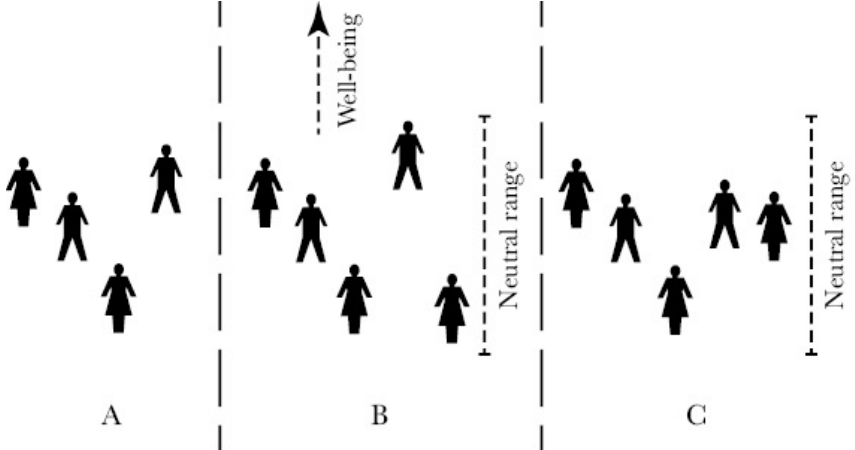
\includegraphics[width=0.8\textwidth]{3-fig-1} \\
  \scriptsize The well-being of the persons in scenarios A, B and C with corresponding utility functions $u_a$, $u_b$, $u_c$. Person $p$ is the right person in A and the second person from the right in B and C. Person q is the rightmost person in B and C. Copied from \citeNP[p.~177]{broome_2012}.
\end{center}
\end{Counterexample}

There are three scenarios A, B and C. They share the same population, except that one additional person exists in both B and C. In both B and C the additional person has a level of well-being within the neutral range. The argument is structured into two major steps:  

First, scenario A is being compared to scenario B and to scenario C. The additional person can be neglected in this step because the person is within the neutral range. There is one person who is a little bit better off in scenario B than in scenario A. As all other persons have exactly the same level of well-being, it is reasonable that there is a higher welfare in scenario B than in scenario A. Contrarily, there is one person who is a little bit worse off in scenario C than in scenario A. As all other persons have exactly the same level of well-being, it is reasonable that there is a higher welfare in scenario A than in scenario C. As a consequence of these two observations, scenario B has a higher welfare than scenario C. Technically, this conclusion requires transitivity of the betterness relation.  

\begin{Premise}{Transitivity of betterness (P2)}{p2}
$
  u_X(P) > u_Y(Q) \wedge u_Y(Q) > u_Z(R) \\
  \rightarrow
  u_X(P) > u_Z(R)
$
\end{Premise}

Second, scenario B is compared directly to scenario C. Both scenarios comprise the same people, so there is no additional person in either scenario who could be neglected. The person who is not present in scenario A and has therefore been neglected above is much better off in scenario C than in scenario B. This big difference clearly outweighs the difference of the other person’s well-being in favour of scenario B. As there is moreover a lower inequality in scenario C, scenario C has a higher welfare than scenario B. This is in contradiction to the result of step one, so the counter-example refutes the intuition of neutrality, which has been its core assumption.  

Whilst the argument above is intuitively plausible, it has two other important premises \cite[p.~177f]{broome_2012}: First, if in two scenarios all persons have the same level of well-being except for one person who is better off in the second scenario, then the welfare in the second scenario is higher than in the first. Technically, we can say that the second scenario Pareto dominates the first \cite{osborne_1997}. (I will come back to this notion in section \ref{sec:obj1}.)

\begin{Premise}{Pareto domination (P3)}{p3}
  \begin{enumerate}
  \item
    $
      \exists p \in P:
    $ \\
    \hspace*{1cm} $
      u_X(a) > u_Y(p) \ \wedge
    $ \\
    \hspace*{1cm} $
      \forall q \in P \setminus \{p\}: u_X(q) = u_Y(q) )
    $ \\
    \hspace*{.5cm} $
      \rightarrow
      u_X(P) > u_Y(P) 
    $
  \item
    $
      \exists p \in P:
    $ \\
    \hspace*{1cm} $
      u_X(a) < u_Y(p) \ \wedge
    $ \\
    \hspace*{1cm} $
      \forall q \in P \setminus \{p\}: u_X(q) = u_Y(q) )
    $ \\
    \hspace*{.5cm} $
      \rightarrow
      u_X(P) < u_Y(P) 
    $
  \end{enumerate}
\end{Premise}

Second, if in two scenarios with the same population the sum of individual well-being is higher in the second scenario, and at the same time the inequality of the distribution of well-being is lower in the second scenario, then the second scenario is better in terms of welfare than the first. I call this the fair aggregation principle. 

\begin{Premise}{Fair aggregation principle (P4)}{p4}
  \hspace*{.5cm} $
    \sum_{p\in P} u_X(p) > \sum_{p\in P} u_Y(p) \ \wedge
  $ \\
  \hspace*{.5cm} $g_X(P) < g_Y(P)
  $ \\
  $
    \rightarrow u_X(P) > u_Y(P)
  $ \\
  with suitable inequality function $g$ (see below).
\end{Premise}

There are various ways to measure inequality, and the details need not concern us here. An excellent survey of one-dimensional inequality measures – as applied in welfare economics – is given in \citeNP{sen_1997}. The most prominent inequality measure is probably the Gini coefficient (see \citeNP{ceriani_2012}). Both of these premises appear to be very plausible, and they are dubbed "hard-to-doubt assumptions" in \citeNP[p.~176]{broome_2012}. 

The following proof concisely sums up the argument presented above. It makes use of the technical premises (P...) and the assumptions that make up the setting of the counter-example (A...). We can infer from the contradiction in (C8) that at least one of the premises and assumptions must be false. The assumptions merely describe the setting of the scenarios as depicted in the figure above. They are simply the assumptions making up the counter-example and there is no reason to doubt them within this proof. Moreover, premises (P2), (P3) and (P4) appear to be very plausible. As a consequence, the intuition of neutrality must be the false premise. 

\begin{Proof}{The argument against neutrality}{arg}
\begin{enumerate}
\item[(C1)] \hspace{1cm}
$(P3) \wedge (A1) \wedge (A2) \Rightarrow \ u_B(P_0) > u_A(P_0)$
\item[(C2)] \hspace{1cm}
$(P3) \wedge (A1) \wedge (A3) \Rightarrow \ u_C(P_0) < u_A(P_0)$
\item[(C3)] \hspace{1cm}
$(C1) \wedge (P1) \wedge (A4) \Rightarrow \ u_B(P_0 \cup P_+) > u_A(P_0)$
\item[(C4)] \hspace{1cm}
$(C2) \wedge (P1) \wedge (A4) \Rightarrow \ u_C(P_0 \cup P_+) < u_A(P_0)$
\item[(C5)] \hspace{1cm}
$(C3) \wedge (C4) \wedge (P2) \Rightarrow \ u_B(P_0 \cup P_+) > u_C(P_0 \cup P_+)$
\item[(C6)] \hspace{1cm}
$(A1) \wedge (A5) \Rightarrow \sum_{x\in P_0} u_B(x) < \sum_{x \in P_0} u_C(x)$
\item[(C7)] \hspace{1cm}
$(C6) \wedge (P4) \wedge (A6) \Rightarrow  \ u_B(P_0 \cup P_+) < u_C(P_0 \cup P_+)$
\item[(C8)] \hspace{1cm}
$(C4) \Leftrightarrow \neg (C7)$
\item[(C9)] \hspace{1cm}
$(C8) \wedge (A1-A6) \wedge (P2) \wedge (P3) \wedge (P4) \Rightarrow \neg (P1)$
\end{enumerate}
\end{Proof}

There are two major implications if this argument holds and the intuition of neutrality is inconsistent (cf. \citeNP[p.~411]{broome_2005}: 

\begin{enumerate}
\item We as a society would have to develop a different, consistent principle to replace the intuition. We do not even currently know whether population changes should be evaluated as positive or as negative, just that they cannot simply be evaluated as neutral. The finding of a new principle with wide acceptance would certainly present a major societal task and require many years of discourse. 
\item As soon as we had found a suitable principle, we would need to gain better knowledge of which actions lead to which consequences with respect to population changes. Only then would we probably be able to apply a principle which is not based on neutrality. This requires new scientific analysis and simulation because such predictions have often been omitted in the past (\citeNP[p.~402]{broome_2005}; \citeNP[p.~115f]{broome_2012}). 
\end{enumerate}

\citeNP{broome_2004} develops five possible responses to the argument against neutrality (see the overview on p.~149). Accordingly, one of the following alternative propositions could be embraced: 

\begin{enumerate}[(a)]
\item intransitivity of the betterness relation 
\item conditional goodness \todo{what this mean}
\item relative goodness \todo{what this mean}
\item indeterminacy or vagueness of the betterness relation \todo{how this different from uncertainty}
\item a single neutral level
\end{enumerate}

The transitivity of the betterness relation (P2) is plausibly defended in (a) -- see \citeNP[p.~151f]{broome_2004}. 
(P3) and (P4) have not been discussed so far. This is what I will do in section \ref{sec:obj1}. 
Section \ref{sec:obj2} will be very similar to what \citeNP{broome_2004} develops with regard to proposition (d), but it will also be compatible with proposition (e). 
I will pursue a somewhat related approach to (b) and (c), focused more on justification, in section \ref{sec:obj3}.\todo{aha echt?}